\documentclass[12pt]{article}

% Language setting
% Replace `english' with e.g. `spanish' to change the document language
\usepackage[english]{babel}

% Set page size and margins
% Replace `letterpaper' with `a4paper' for UK/EU standard size
\usepackage[letterpaper,top=2cm,bottom=2cm,left=1cm,right=1cm,marginparwidth=1.75cm]{geometry}

% Useful packages
\usepackage{amsmath}
\usepackage{graphicx}
\usepackage[colorlinks=true, allcolors=blue]{hyperref}
\usepackage{graphicx}%
\usepackage{multirow}%
\usepackage{amsmath,amssymb,amsfonts}%
\usepackage{amsthm}%
\usepackage{mathrsfs}%
\usepackage[title]{appendix}%
\usepackage{xcolor}%
\usepackage{textcomp}%
\usepackage{manyfoot}%
\usepackage{booktabs}%
\usepackage{algorithm}%
\usepackage{algorithmicx}%
\usepackage{algpseudocode}%
\usepackage{listings}%
\usepackage[justification=centering]{caption}%
\usepackage[greek,english]{babel}%
\usepackage[verbose]{placeins}%
\usepackage{forest}%
\usepackage{tikz}%
\usepackage{mathtools}%
\usepackage[demo]{graphicx}%
\usepackage{caption}%
\usepackage{subcaption}%
\usepackage{pgfplots}%
\usepackage{cite}
\usepackage[sorting=none]{biblatex} %Imports biblatex package
\addbibresource{sn-bibliography.bib} %Import the bibliography file
\title{Computational Fluid Dynamics}
\author{\fnm{Pranav } \sur{Sridhar} MM22B046}



\begin{document}
\maketitle
\begin{center}
\paragraph{MM2041 Assignment}

\end{center}

\begin{center}
\paragraph{Metallurgical and Materials Engineering, IIT Madras}
\end{center}
\abstract{\textbf{Purpose:} This assignment serves to provide a entry into exploring the vast fields of Computational Fluid Dynamics, which will be referred to as CFD, with strong emphasis on foundational examples and motives. The goal is to provide readers with an understanding of why this field of study exists and a solid understanding of the methods employed.

\textbf{Methods:} This assignment will cover the basics of common CFD methods and techniques. I will do my best to ensure that this will be useful for anyone, regardless of their understanding of fluid dynamics. The methods discussed will be broken down to first principles and the main goal will be to provide rationale as to the existence of these methods and a strong mathematical background for the same.

\textbf{Conclusions:} The assignment will have covered in a sequential manner the history, purpose, fundamentals, common practices and latest developments of CFD research. The assignment also presents readers with a tutorial of sorts, into the basics of fluid simulations and all work presented can be accessed on Github. Readers will have an appreciation for CFD and all the principles that are inherent to it.
 }

\clearpage
\tableofcontents
\clearpage
\section{Introduction}

The Introduction section expands on the background of CFD. It seeks to cover some significant milestones in research, while outlining the thought process and principles behind these advancements. It is crucial to understand this as it provides a solid backbone understanding of how things are the way they are today. To be a good problem solver, it is important to always trace back to the fundamental building blocks of the problem. Hence to facilitate that method of thought we will cover some of these milestones.

\subsection{History}

\subsubsection{Ancient Times}
Understanding fluid dynamics has been something humans have been trying to do since the start of civilisations. Most of these civilisations resided near fast flowing water bodies i.e rivers. They designed irrigation systems, boats, weapons and had an understanding of how fluids behaved. The Egyptians recorded the year rise of level of the Nile. They knew from their irrigation system that Narrower meant Faster, something we formally study as $A_{1} V_{1} = A_{2} V_{2}$ which relates the area of cross section of a flow of fluid with its velocity. The Egyptians invented a Screw Pump \cite{bib1} which dates back to before 3 B.C. It was the first ever positive displacement water pump, that utilised tubes wound around a cylinder, which when spun brought up water along with it. 
\subsubsection{Pre Classical Mechanics}
These were the times of Aristotle, Archimedes and Da Vinci. Majority of foundations for static understanding of fluids were set in this time. \\ 

The earliest forms of mathematical and scientific basis for the same were also established. Archimedes (287 BC - 212 BC) touted as the Father of Fluid Statics figured out why bodies behave the way they do in fluids. Why some float, why some sink? \\

He formulated some key ideas we still use in every fluid dynamics problem - 
\begin{itemize}
    \item Fluids are continuous and cannot have "empty" spaces
    \item Concept of Hydrostatic pressure
    \item Concept of equilibrium of fluids at same weight and height from the centre of the Earth
    \item Archimedes Principle - "The upward buoyant force that is exerted on a body immersed in a fluid, whether partially or fully submerged, is equal to the weight of the fluid that the body displaces and acts in the upward direction at the center of mass of the displaced fluid" $F_{b}= - \rho g h$ \cite{bib3}
    \item Of course, the famous $\textgreek{εύρηκα} (Eureka)$ is said to have originated with Archimedes in a bathtub finally having figured it all out.
\end{itemize}
Da Vinci is credited with the formulation of the Velocity-Area law $Av = Constant$, a continuity equation.  He also had this drawing the earliest observation as shown in Figure \ref{fig:fig3} of a certain phenomenon, we still cant entirely understand - Turbulence! 

\begin{figure}[hbt!]
  \centering
  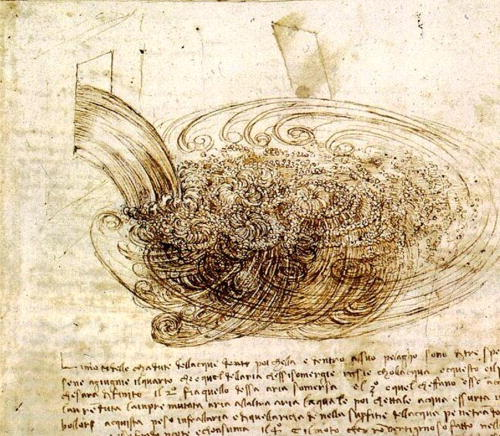
\includegraphics[width=4cm]{plot1.jpeg}
  \caption{La Turolenza - Da Vinci \cite{bib2}Drawing of turbulent flows \label{fig:fig3}}
\end{figure}
\FloatBarrier 
\subsubsection{Newton and Euler Era}
Newton came along with the equations of motion and set the founding stones for Classical Mechanics. We will find great relevance in his 2nd law (1), which can be thought of as the real start of all fluid dynamic situations. Newton also studied the behaviour of Newtonian Fluids and formulated the definition of viscous friction \cite{bib4} as in (2)

\begin{equation}
    \frac{d(m \Vec{V})}{dt}= \Vec{F} 
\end{equation}


\begin{equation}
    \tau_{12} = \mu \frac{\partial u}{\partial y}
\end{equation}

This was the time Euler (1757) stepped in and generalised Newton's second law using the continuity equation (derived from conservation of mass, thank you Da Vinci)(3) into something that can be reproducible and he formulated the Euler's Equation (4) for an inviscid, incompressible fluid. We can derive this using a control volume method $\nabla V = dx dy dz$. We then calculate the net force on this infinitesimally small box and then plug it into our force and continuity equations.

\begin{equation}
    \frac{\partial \rho}{\partial t} + \nabla \cdot(\rho \cdot \Vec{V}) = 0
\end{equation}
\begin{equation*}
    F_{net} = f_{body} +f_{surface}
\end{equation*}
Making using of the material derivative, Euler derived the first differential equation in this field of study! A remarkable equation with each term having such intricate implications.
\begin{equation*}
    F_{net} =  \rho \Vec{g} - \nabla p 
\end{equation*}
\begin{equation}
    \rho [ \frac{\partial \Vec{V}}{\partial t} + (\Vec{V} \cdot \nabla)\Vec{V}] = - \nabla p + \rho \Vec{g}
\end{equation}

\subsubsection{Navier - Stokes}
Navier and Stokes, building upon on each other finally presented the Navier-Stokes Equation \cite{bib4} we know of - 
\begin{equation}
    \rho [ \frac{\partial \Vec{V}}{\partial t} + (\Vec{V} \cdot \nabla)\Vec{V}] = - \nabla p + \Vec{f}_{b} + \mu \nabla^{2} \Vec{V} + \frac{1}{3}\mu \nabla (\nabla \cdot \Vec{V})
\end{equation}
We will skip over the exact derivation of the NS equation, as it has been extensively documented. However, in a later section, the NS equation will be thorougly investigated and intuitively.

The key differences in Euler's form and NS form is the additional viscous term and another term included in to account for the effects of fluid compressibility. In Euler's form the compressibility term goes to 0.
\subsection{Present}
Navier-Stokes for an incompressible fluid can be modelled as 4 partial differential equations, 3 from (5) for each dimension and 1 from the continuity equation $ \nabla \cdot V = 0$. Here we have 4 equations and we are solving for 4 unknowns, namely the three velocity components and the pressure.

There are many well established solutions Navier-Stokes equation. So at this point, we feel a sense of completeness, that we have modelled fluid flow and all the work is done! Unfortunately that is too good to be true, as we have solved for a very specific set of the Navier Stokes equation. There are a whole huge bunch of them we have not even come close to achieving an analytical solution. 

\subsubsection{Million Dollar Problem}

Werner Heisenberg: "When I meet God, I am going to ask him two questions. Why relativity and why turbulence? I really believe he will have an answer for the first."

The Clay Mathematics Institute \cite{bib5} has offered a cash prize of one million dollars to anyone who can demonstrate that the solutions of the Navier-Stokes equations remain bounded and physically realistic under ALL flow conditions. 

The ALL in the problem statement above holds a lot of significance. Every PDE is bound by its initial conditions, geometry and assumptions. We have solutions for well-behaved, incompressible, laminar flow. Tweak a few of those initial conditions and things get very, very messy. There are mainly 3 reasons why the analytical global regularity is hard (potentially impossible?) - 
\begin{itemize}
\item Non-linearity
\begin{itemize}
    \item A first order PDE \cite{bib6} is said to linear if it is of the form $ P(x,y) p + Q(x,y)q = R(x,y)z + S(x,y) $ . Example: yp - xq = xyz +x
    \item If a function $u(x,y)$ has every term linear, then it is linear. A term is linear if it can be written as $g(x,y)Du$ where D is some differential operator. Basically $u$ can appear at most once per term. Hence for example, something like $x\frac{\partial u}{\partial y} - y \frac{\partial u}{\partial x}$ is linear. Whereas $u^{2}$ is not linear.
    \item The reason these non-linear forms are hard to solve is - they cannot be generalised into methods. Each problem needs a separate form of study.
    \item We generally employ a strategy of finding two solutions and then by linearity we say that the sum of the two solutions is a more general solution. We cannot do this for non-linear cases, hence for these reasons, it is much more difficult to deal with.
\end{itemize}

\item Turbulence and Issues with Scale
\begin{itemize}
    \item Taking the Navier Stokes equation, we have two force terms. 
    \item Let us analyse the example of Prandtl trip wire. First, we take flow around a perfectly smooth sphere. Then we use a very thin wire, whose diameter is less than $1/100$ of the sphere diameter.
    \item The flow is dramatically different. Small disturbances causes big changes.
\begin{figure}[hbt!]
\centering
\begin{subfigure}{0.4\textwidth}
  \centering
  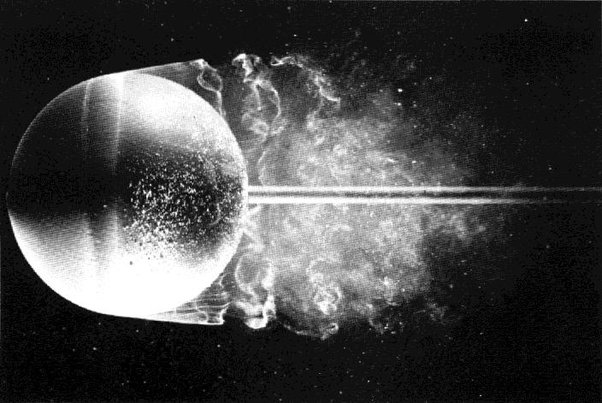
\includegraphics[width=.5\linewidth]{plot2.jpeg}
  \caption{Thick Wire}
  \label{fig:sub1}
\end{subfigure}%
\begin{subfigure}{0.4\textwidth}
  \centering
  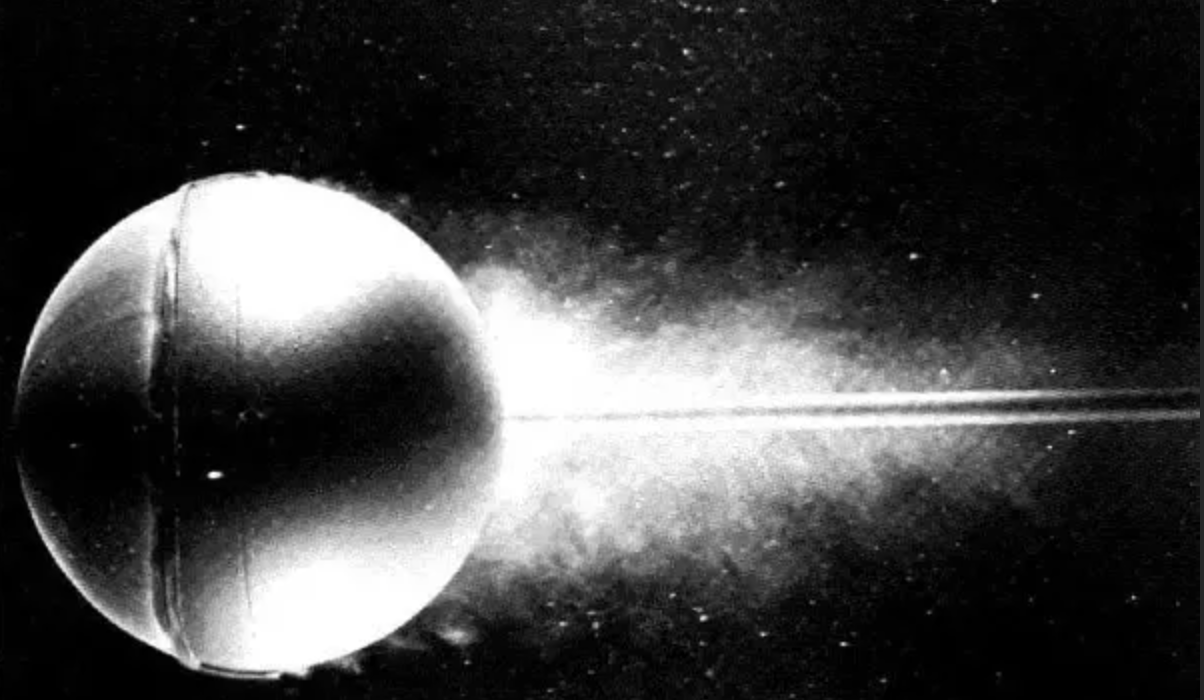
\includegraphics[width=.5\linewidth]{plot33.png}
  \caption{Thin Wire}
  \label{fig:sub2}
\end{subfigure}
\caption{A Comparison of flow patterns}
\label{fig:test}
\end{figure}
\FloatBarrier 
    \item In many real-life cases, they are hard to analytically (or numerically) solve because small but non-zero viscosity leads to chaotic behaviour on spatial scales smaller than the domain size, i.e. turbulence.
    \item Chaotic behaviour means it is incredibly sensitive to initial conditions. Like the example we saw, even small disturbances cause big changes. So we need extremely small resolutions. It would be like mapping the entire Ganga river in the scale of a centimeter.
    \item Turbulence is the reason we can't predict the weather past 7 days and why airplanes can't account for turbulence beforehand. 

\end{itemize}
\end{itemize}
\subsubsection{Power of Computation}
Thus far, we have shown that the research and work done in this field is extensive, but still it isn't enough. We still can't find an analytical solution. If this was a field of study that didn't have direct human applications, we would've probably called it quits by this points. However, fluid dynamics applications are everywhere, truly. We will go over some examples later.

So we are at a junction where we need solutions but we can't analytically or numerically get them. One might suggest experimentation. This will work, but for a small number of cases. Most real world applications are extremely difficult to practically experiment and take readings with errors.

This leads us to the last resort - Simulation. This path of going from the bare basic fundamentals of fluids, we have reached a stage where we need to computationally predict how certain fluid set ups will behave.

CFD has allowed us to design, engineer and invent life altering technologies in many industries. 

\begin{itemize}
    \item Design of aircrafts and automobiles
    \item Weather forecasting and atmospheric modelling
    \item Chemical Engineering processes
    \item Any form of system that utilises cooling systems
\end{itemize}

CFD was born in Los Alamos as part of the T3 group, pioneered by Fracis H. Harlow in 1957. Since then, CFD has penetrated almost all industries, really highlighting the power of computation.

To be able to hypothesise, experiment, evaluate any methodology for most industry problems all from a computer with negligible error is a superpower. Significantly cheaper, faster and more accurate than any other feasible method.

\section{Diving Deep into CFD }
Thus far, we have explored the reasons and historical significance for the existence of CFD. This brings us to the question, what exactly is CFD? \cite{bib7}\cite{bib8}\cite{bib9}\cite{bib10}
\subsection{What is CFD?}
We convert the continuous problem domain into a discrete domain using a grid. We discretize the problem because it converts the governing equations into a set of simple equations. There are a few methods of discretization that are commonly used. We will focus on mesh methods. 
\begin{center}
\begin{figure}
    \begin{forest}
   [Mesh Methods Steps, rectangle, draw
       [Meshing, rectangle, draw
           [Divide Domain into Smaller Regions, rectangle, draw
               [Triangles, Rectangles (2D), rectangle, draw]
               [Tetrahedrons, Hexahedrons (3D), rectangle, draw]
           ]
       ]
       [Discretization of Governing Equations, rectangle, draw
           [Finite Differences, rectangle, draw
               [Forward Difference, rectangle, draw]
               [Backward Difference, rectangle, draw]
               [Central Difference, rectangle, draw]
           ]
           [Finite Volumes, rectangle, draw]
           [Finite Elements, rectangle, draw]
       ]
   ]
   [Meshfree Methods, rectangle, draw
       [Smooth Particle Hydrodynamics (SPH), rectangle, draw]
       [Finite Pointset Method (FPM), rectangle, draw]
   ]

    \end{forest}

    \caption{Steps in Meshing}
    \label{fig:enter-label}
\end{figure}
\end{center}

Take the case of pressure $p$ in an 1D domain, the function would be
\begin{equation*}
    p=p(x), 0 < x < 1
\end{equation*}

In the discrete case, we would model it as

\begin{equation*}
    p_{i} = p(x_{i}), i = 1,2,\dots, N
\end{equation*}
\

\begin{center}

\begin{tabular}{cc}
\textbf{Continuous Domain} & \textbf{Discrete Domain} \\
$0 \leq x \leq 1$ & $x = x_1, x_2, \ldots, x_N$ \\
\\
\begin{tikzpicture}
    \draw[thick] (1,0) -- (5,0);
    \fill (1,0) circle (2pt) node[below] {$x=0$};
    \fill (5,0) circle (2pt) node[below] {$x=1$};
\end{tikzpicture}
&
\begin{tikzpicture}
    \draw[thick] (1,0) -- (5,0);
    \foreach \x in {1,2,3,4,5}
        \fill (\x,0) circle (2pt) node[below] {$x_\x$};
    \fill (5,0) circle (2pt) node[below] {$x_N$};
    \draw[thick,->] (3,0) -- (3,0.5) node[above] {Grid point};
\end{tikzpicture} \\
\\
Coupled PDEs + boundary & Coupled algebraic eqs. in \\
conditions in continuous & discrete variables \\
variables &
\end{tabular}
\end{center}

After dividing the domain into discrete points, the function now only takes values at these specific grid points. In an appropriate CFD solution, we can just solve for the relevant flow variables only at the grid points. Here is where that resolution comes into play, since we  struggle with coming up with a solution are high resolutions, we can find the values at the grid points and interpolate to non-grid points. We approximate our continuous variables $p, \Vec{V}$ to discrete variables $p_{i}, \Vec{V}_{i}$. This discrete system is a large set of coupled, algebraic equations in discrete variables. Solving this discrete system requires a very large number of calculations. Hence we send the Matrix Inversion problem to the computer to try and solve.
\subsection{Discretization with Finite-Difference Method}
\subsubsection{Initial Geometry and conditions}
For simplicity, we will stick to our 1D scenario. 

\begin{equation}
    \frac{\partial u}{\partial x} + u^{m} = 0; \quad 0 \leq x \leq 1; \quad u(0) = 1
\end{equation}

Let's take the linear case m=1. 
\begin{center}
    

\begin{tikzpicture}
    \draw[thick] (0,0) -- (6,0);
    \draw[<->] (2,0.5) -- (4,0.5) node[midway, above] {$\Delta x=1/3$};
    \fill (0,0) circle (2pt) node[below] {$x_1 = 0 $};
    \fill (2,0) circle (2pt) node[below] {$x_2 = 1/3$};
    \fill (4,0) circle (2pt) node[below] {$x_3 = 2/3$};
    \fill (6,0) circle (2pt) node[below] {$x_4 = 1$};
\end{tikzpicture}
\end{center}

Now since we discretized it, the original governing equation is valid at grid points, we have
\begin{equation*}
    (\frac{du}{dx})_{i} + u_{i} = 0
\end{equation*}
Now we need some expression for $(\frac{du}{dx})_{i}$, we use Taylor series approximation:
\begin{equation*}
    u_{i-1}  = u_{i} - \Delta x (\frac{du}{du})_{i} + \mathcal{O}(\Delta x^{2})
\end{equation*}

We have an expression for $(\frac{du}{dx})$. We exlude the higher order truncation error terms. We have a first order accurate solution.
\begin{equation}
    \frac{u_i - u_{i-1}}{\Delta x} + u_i = 0
\end{equation}

We can now appreciate how we went from a differential equation to a set of algebraic equations. 
\subsubsection{Assembly of Discrete System}
We will now rearrange the terms, 
\begin{equation*}
    -u_{i-1} + (1+\Delta x)\space  u_{i} = 0
\end{equation*}
Expanding these for grid points $i = 2,3,4$ $(x_i)$,
\begin{equation}
    -u_{1} + (1+\Delta x)\space u_{2} = 0 \quad (i=2)
\end{equation}
\begin{equation}
    -u_{2} + (1+\Delta x)\space  u_{3} = 0 \quad (i=3)
\end{equation}
\begin{equation}
    -u_{3} + (1+\Delta x)\space  u_{4} = 0 \quad (i=4)
\end{equation}

We can immediately see that at the left boundary $(i=1)$ discrete equation cannot be applied since $u_{i-1}$ isn't defined here. We use boundary condition to get

\begin{equation*}
    u_1 = 1
\end{equation*}

Equations (8) - (10) form a system of 4 simultaneous algebraic equations $u_1, u_2, u_3 and u_4$. 

\begin{equation}
\begin{bmatrix}
1 & 0 & 0 & 0\\
-1 & 1+\Delta x & 0 & 0\\
0 & -1 & 1+\Delta x & 0\\
0 & 0 & -1 & 1+\Delta x
\end{bmatrix}
\begin{bmatrix}
u_1\\
u_2\\
u_3\\
u_4
\end{bmatrix}
=
\begin{bmatrix}
1\\
0\\
0\\
0
\end{bmatrix}
\end{equation}

Hence we see that we now have a combination of discrete equations and boundary conditions. The number of equations is equal to the number of independent discrete variables.

\subsubsection{Solution of Discrete System}
 The Discrete system is of the AU = B, we can invert A and solve for U = $A^{-1}$B.

 In our example, we obtain the following
\begin{equation*}
    u_1 =1 \quad u_2 = 3/4 \quad u_3 = 9/16 \quad u_4 = 27/64
\end{equation*}

Solving (6), we get the exact form of $u$.

\begin{equation*}
    u_{exact} = e^{-x}
\end{equation*}
\begin{center}
\begin{tikzpicture}
\begin{axis}[
    xlabel=$x$,
    ylabel=$u$,
    xmin=0, xmax=1,
    ymin=0.4, ymax=1,
    legend pos=north west,
    cycle multi list={
        red, solid, mark=o\\
        black, dashed
    }
]
\addplot+[mark options={solid}] coordinates {
    (0, 1)
    (0.33, 0.75)
    (0.66, 0.5625)
    (1, 0.4218)
};
\addplot+[mark options={solid}] coordinates{
    (0,1)
    (0.25,0.8)
    (0.5,0.64)
    (0.75, 0.512)
    (1,0.4096)
};
\addlegendentry{Numerical solution N=4 }
\addplot+[no marks] {exp(-x)};
\addlegendentry{Exact solution }
\addlegendentry{Numerical Solution N=5}
\end{axis}
\end{tikzpicture}
\end{center}
Now we have a working, rudimentary understanding of how a general finite differences method of discretization will go about. However there are quite a few intricacies here important to put some thought into -
\begin{itemize}
    \item The error between exact function and approximation gets lesser and lesser as N $\xrightarrow{}\infty$. This error exists because in our Taylor series approximation we neglected higher order terms.
    \item In production commercial CFD software, the actual process of inverting the matrix is done iteratively (we will discuss this next) and not with a simple Gauss Jordan Elimination method. This is because the matrix is quite sparse (filled with 0s) hence it makes sense to store only the required values to be memory efficient. 
    \item On large scales, parallelization techniques will need to be used as the number of operations increases and increases. Running it on a regular CPU with no special techniques will take a long time and will be very inefficient.

\end{itemize}

\subsubsection{Dealing with Non-linearity with Iterative Solvers}
As we have discussed, solving non-linear cases of the NS equation leads to a lot of mathematical problems. Let us take our example from eq (6), with $m = 2$.

\begin{equation}
    \frac{\partial u}{\partial x} + u^{2} = 0; \quad 0 \leq x \leq 1; \quad u(0) = 1
\end{equation}

Approximating to the first order like we did previously in eq (7), we arrive at 
\begin{equation}
    \frac{u_i -u_{i-1}}{\Delta x} + u^{2}_i = 0
\end{equation}
Now, we have a pesky $u^{2}_i $ term making this algebraic equation non-linear. 

The way we will deal with nonlinearity is by linearizing the equation about $guess value$ of the solution and to iterate until the guess agrees with the solution to a specified tolerance level. 

Let $u_gi$ be the guess $u_i$, we define
\begin{equation}
    \Delta u_i = u_i - u_{gi}
\end{equation}
Rearranging and squaring to be able to approximate $u_{i}^{2}$, we get
\begin{equation}
    u_{i}^{2} = u^{2}_{gi} +2u_{gi}\Delta u_{i} + (\Delta u_{i})^{2}
\end{equation}

Neglecting $\Delta u_{i}^{2}$ term, we get the approximation as

\begin{equation*}
    u_{i}^{2} \approx 2u_{gi} u_{i} - u^{2}_{gi}
\end{equation*}

The finite-difference approximation in eq (13) becomes,

\begin{equation}
    \frac{u_{i} - u_{i-1}}{\Delta x} + 2u_{gi}u_{i} - u^{2}_{gi} = 0
\end{equation}

The error due to linearization is in the order of $\Delta u^{2}$. It tends to zero as $u_{g} \xrightarrow{} u$.

Now that we have the required expressions, we can begin getting the guess values $u_g$ at the grid points. We do this iteratively by starting with an initial guess value in the first iteration. In each iteration, the $u$ value obtained in the previous iteration is used as the guess value. 
\\
\begin{center}
    

Iteration 1: $u^{(1)}_{g}$ = Initial guess \\
Iteration 2: $u_{g}^{(2)} = u^{(1)}$ \\
$\dotsc$ \\
Iteration l: $u^{(l)}_g  = u^{(l-1)}$ \\
\end{center}
We continue the iterations until convergence.

We can assemble eq (12) as below, 

\begin{equation}
\begin{bmatrix}
1 & 0 & 0 & 0\\
-1 & 1+2 \Delta x u_{g2} & 0 & 0\\
0 & -1 & 1+2 \Delta x u_{g3} & 0\\
0 & 0 & -1 & 1+2 \Delta x u_{g4}
\end{bmatrix}
\begin{bmatrix}
u_1\\
u_2\\
u_3\\
u_4
\end{bmatrix}
=
\begin{bmatrix}
1\\
\Delta x u^{2}_{g2}\\
\Delta x u^{2}_{g3}\\
\Delta x u^{2}_{g4}
\end{bmatrix}
\end{equation}

In any useful real world application this matrix would be of order of million size (albeit sparse for the most part). We need to invert the matrix using an iterative scheme.

Let us take eq (16) and rearrange the terms of the finite-difference approximation at grid point i, so we get an expression for $u_i$ in terms of the values at neighboring grid points and guess values
\begin{equation}
    u_i =\frac{ u_{i-1} + \Delta x \space u^2_{gi}}{1 + 2 \Delta x \space u_{gi}}
\end{equation}

If at a specific iteration level, the neighbouring value isn't available, we use the guess value for it. We update $u_4$, then $u_3$ and finally $u_2$ in each iteration. In the $m^{th}$ iteration, $u^{(l)}_{i-1}$ won't be there when updating $u^m_{i}$, so we use the guess value $ u^{(l)}_{g_{i-1}}$
\begin{equation}
    u_i^{(l)} = \frac{u_{g_{i-1}}^{(l)} + \Delta x u^{(l)^{2}}_{g_{i}}}{1+ 2 \Delta x u^{(l)}_{g_{i}}}
\end{equation}

We have effectively found approximate solution for the matrix inversion during each iteration but in the process have greatly reduced the memory required for inversion. We have coupled the iteration to handle nonlinear terms with the iteration for matrix inversion into a single iteration process. This will eventually converge and iterate into the exact solution for the inversion since error introduced by the guess values also goes to 0.

As $u_{g} \xrightarrow{} u$, the errors in linerization tend to 0. The obvious question to ask would be, when do we stop iteration? We define a residual R as the root-mean-squared value of the difference between the real and guess values on the grid
\begin{equation}
    R = \sqrt{\frac{\sum_{i=1}^{N} (u_i - u_{gi})^{2}}{N}}
\end{equation}
\subsubsection{Finite Volume Method}
The basic idea is very similar to finite differences. We split the grid into $\textit{cell}$ and grid points as $\textit{node}$. Integral form of the conservation equations are applied to the control volume defined by a cell to get the discrete equations for the cell. Integral form for steady, incompressible flow is as eq (5). This signifies the fact that net volume flow into control volume is zero.
\begin{equation}
    \int_{S} \Vec{V} \cdot \hat{n}\, dS = 0
\end{equation}

Let us take a rectangular cell like below, 

\begin{center}
    

\begin{tikzpicture}
    % Draw the rectangle
    \draw (0, 0) rectangle (4, 2);
    
    % Draw the dot in the center
    \fill (2, 1) circle (2pt);
    \node[below] at (2, 0) {Face 2 $(u_{2}, v_{2})$};
    \node[above] at (2, 2) {Face 4 $(u_{4}, v_{4})$};
    \node[left] at (0, 1) {Face 1 $(u_{1}, v_{1})$};
    \node[right] at (4, 1) {Face 3 $(u_{3}, v_{3})$};

\end{tikzpicture}
\end{center}
The velocity at face $i$ is 
\begin{equation*}
    \Vec{V}_{i} = u_{i} \hat{i} + v_{j} \hat{j}
\end{equation*}

Using (21) to the control volume gives us 
\begin{equation}
-u_1\Delta y - v_2\Delta x + u_3\Delta y + v_4\Delta x = 0
\end{equation}
We have successfully discretised the continuity equation for this cell. Mass is conserved in the cell. The same forms can be obtained for momentum and energy equations. Let us take some time to ponder about what the exact differences are between finite-differences and finite-volume methods. Table 1 has covered the key differences.\\
\FloatBarrier 

\begin{table}
\centering

\begin{tabular}{|p{0.2\linewidth}|p{0.3\linewidth}|p{0.3\linewidth}|}
\hline
\textbf{ Basis} & \textbf{Finite-Difference Method} & \textbf{Finite-Volume Method} \\
\hline
Domain Discretization &
\begin{itemize}
  \item Grid of nodes or points
  \item All the variables are defined at the nodes
\end{itemize} &
\begin{itemize}
  \item Divided into control volumes or cells
  \item All variables are averaged values over the cell
\end{itemize} \\
\hline
Equation Discretization &
\begin{itemize}
  \item Finite-difference approximations are used to get derivatives at the nodes
  \item We have to solve algebraic equations at every node
\end{itemize} &
\begin{itemize}
  \item Equations are integrated over the control volume
\end{itemize} \\
\hline
Conservation Properties &
\begin{itemize}
  \item Conservation laws aren't explicitly directly satisfied
  \item We may need additional constraints 
\end{itemize} &
\begin{itemize}
  \item Defined with the conservation laws being satisfied
  \item Better for problems where we have conservation laws used directly.
\end{itemize} \\
\hline
Geometric Flexibility &
\begin{itemize}
  \item Structured grids 
  \item Complex geometries get tedious to define and use
\end{itemize} &
\begin{itemize}
  \item Handles complex geometries 
  \item Uses unstructured or body-fitted grids
\end{itemize} \\
\hline
\end{tabular}
\caption{Comparison of Finite-Difference and Finite-Volume Methods}
\label{tab:comparison}
\end{table}


\section{Lattice Boltzmann Method}
The novelty of this method lies in the fact that it is able to simulate the effects of Navier Stokes, but without needing to solve it. It started in early 1990s, where scientists tried to approach the problem from a molecular level. \\

Suppose the fluid is an ideal gas at temperature $T$. All molecules have thermal velocities $\Vec{v}$ that are governed by the Boltzmann distribution of statistical mechanics \cite{bib11}\cite{bib12}
\begin{equation}
    D(\vec{v}) = \frac{m}{2\pi k T} e^{\frac{-m \vec{V}^{2}}{2kT}}
\end{equation}
This function will give the probability that a molecule has a particular velocity if it is integrated with the velocity limits. In this method, we discretize both space and time and ensure only particular velocities are allowed. \\
\subsection{Representations}
The grids we choose can be of many types, but we will stick to the $D_{n} Q_{m}$ naming convention. $D_{n}$ represents number of dimensions and $Q_{m}$ represents number of directions the particle moves. A very common one is $D2Q9$. \\

\begin{center}
\begin{tikzpicture}[scale=1.25]
    % Draw the grid
    \draw (0,0) grid (3,3);
    
    % Draw dots in each box
    \foreach \x in {0,1,2}
        \foreach \y in {0,1,2}
            \fill (\x + 0.5, \y + 0.5) circle (2pt);
            
    % Draw arrows
    \draw[->] (1.5, 1.5) -- (2.45,1.5);
    \draw[->] (1.5, 1.5) -- (2.45,2.45);
    \draw[->] (1.5, 1.5) -- (1.5,2.45);
    \draw[->] (1.5, 1.5) -- (1.5,0.55);
    \draw[->] (1.5, 1.5) -- (2.45,0.5);
    \draw[->] (1.5, 1.5) -- (0.5,0.5);
    \draw[->] (1.5, 1.5) -- (0.55,1.5);
    \draw[->] (1.5, 1.5) -- (0.5,2.45);
\end{tikzpicture}
\end{center}
We can describe a set of 9 displacement vectors $e_{i}$ where $i \epsilon [0,8]$. Each $e_{i}$ has x and y components that are -1,0 or 1. We will now seek to find and attach probabilities to each of these directions. We can take a set of weights $w_{i}$ that map to each $e_{i}$. Different scenarios will prompt different probabilities. 

We can draw a parallel between the actual boltzmann probability expression and the one we just derived. 
\begin{equation}
    \int_{- \infty}^{\infty} \int_{- \infty}^{\infty} v^{2}_{x} D(\vec{v}) dv_{x} dv_{y} = \sum^{8}_{i=0} (e_{i,x})^{2} w_{i}
\end{equation}
\subsection{The Algorithm}
We consider the fluid to be a collection of molecules that exist on a lattice. These molecules, over time, move to adjacent cells and collide with other particles. Macroscopic properties of the fluid is then calculated in each cell, simply based on the particles that exist in the cell. The steps are as follows
\begin{itemize}
    \item Streaming
    \item Bouncing
    \item Collision
\end{itemize}
\subsubsection{Streaming}
In every streaming step, all the particles move in their respective directions. Densities change and move to adjacent lattice cells. If a density in the Left direction exists, it will become the Left direction for the Left adjacent cell in the next time step. Stationary densities remain the same.
\begin{figure}[hbt!]
\centering
\begin{subfigure}{0.4\textwidth}
  \centering
  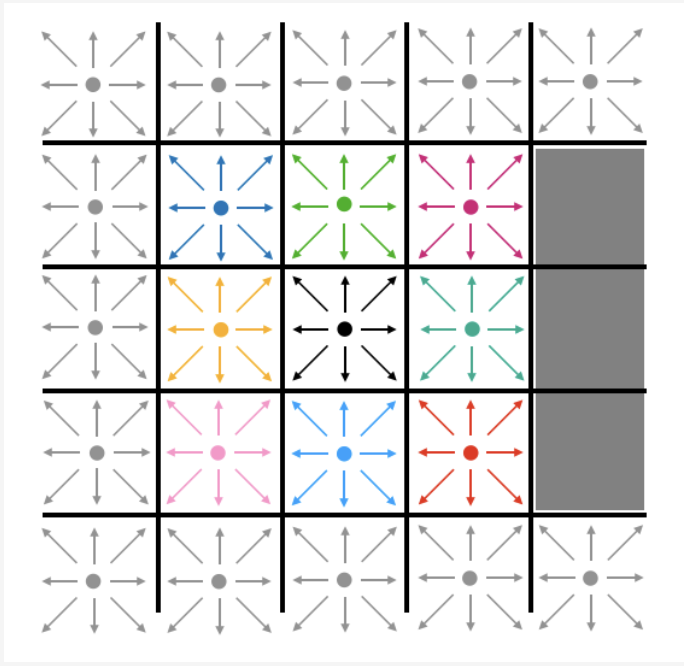
\includegraphics[width=0.9\linewidth]{plot10.png}
  \caption{Before streaming}
  \label{fig:sub1}
\end{subfigure}%
\begin{subfigure}{0.4\textwidth}
  \centering
  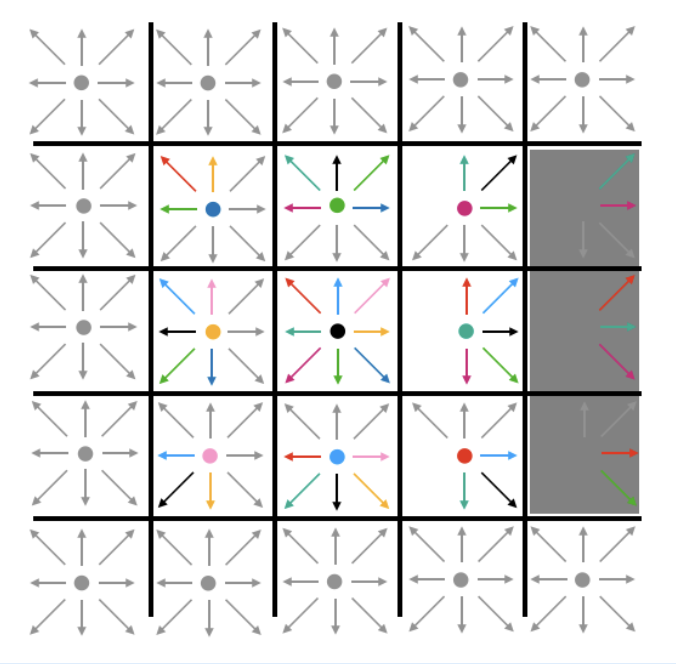
\includegraphics[width=0.9\linewidth]{plot11.png}
  \caption{After streaming}
  \label{fig:sub2}
\end{subfigure}
\caption{Effects of Streaming}
\label{fig:test}
\end{figure}
\FloatBarrier 
\subsubsection{Bouncing}
Now after streaming there will be some densities that are in the barriers. We need a mechanism to reflect them back, as would happen intuitively. So we just reverse their direction and send them back to the cell they came from.
\begin{figure}[hbt!]
\centering
\begin{subfigure}{0.4\textwidth}
  \centering
  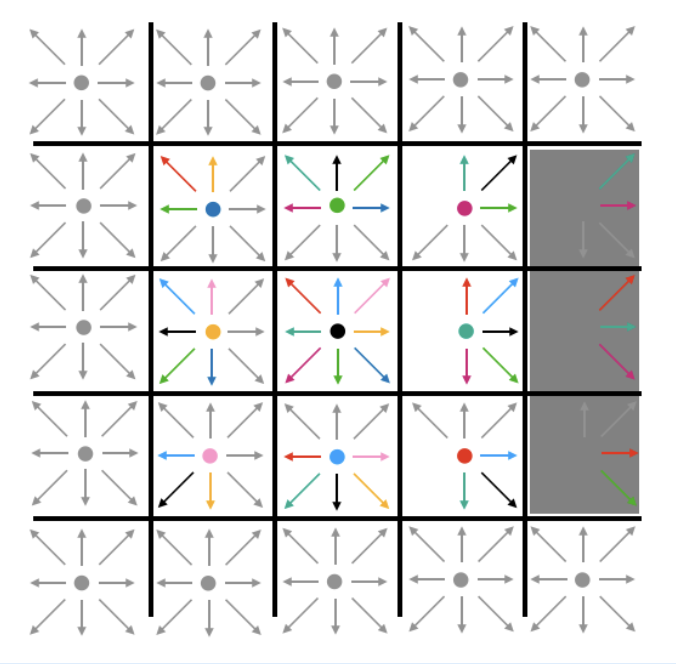
\includegraphics[width=0.9\linewidth]{plot11.png}
  \caption{After streaming}
  \label{fig:sub1}
\end{subfigure}%
\begin{subfigure}{0.4\textwidth}
  \centering
  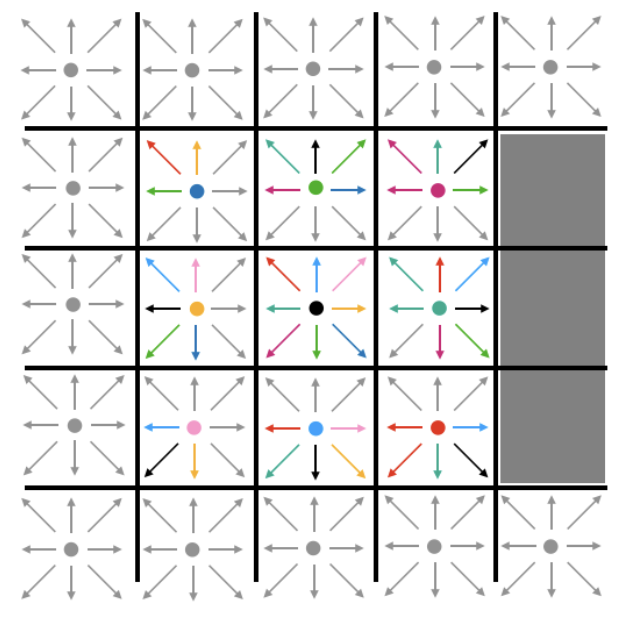
\includegraphics[width=0.9\linewidth]{plot12.png}
  \caption{After Bouncing}
  \label{fig:sub2}
\end{subfigure}
\caption{Effects of Bouncing}
\label{fig:test}
\end{figure}
\FloatBarrier 
\subsubsection{Collisions}
For every lattice site, we compute the macroscopic density $\rho$ and velocities $ u_x$ and $u_y$.
\begin{equation}
    \rho = \sum_{i=0}^{8} n_i
\end{equation} \\

We can calculate the x and y velocity components by averaging the cells x and y velocities.

\begin{equation}
    u_x = \frac{n_E + n_{NE} + n_{SE} - n_{W} - n_{NW} - n_{SW} }{\rho}
\end{equation}
\begin{equation}
    u_y = \frac{n_N + n_{NE} + n_{NW} - n_S - n_{SE} - n_{SW}}{\rho}
\end{equation}

Where N, S, E, W, NE, NW, SE, SW are the 8 directions.

Using these value we can calculate specific expressions for all the 9 densities. We will compute them and then find the $0$ vector that conserves mass. We can then calculate speed, density, curl and update by streaming, bouncing and colliding again.
\subsection{Perspective}
The algorithm is quite simple and can simulate plenty of complicated nonlinear macroscopic phenomena. It is also able to handle many complex boundaries because of the molecular level bouncing. \\

The reason we are discussing it is that it is quite simple to program and the calculation is already derived and is straightforward to represent as matrices. We can obtain density, velocity and pressure values while being easy to process. The LBM method is suitable for parallel compute. However the biggest con is the memory intensive nature of LBM.
\subsection{Implementation}
Running a simulation in python of LBM method for fluid flow with an initial eastward velocity with an Line object in the domain, we get these flow patterns in Figure \ref{fig:images}. 
\begin{figure}[htbp]
    \centering
    \begin{subfigure}[b]{0.45\textwidth}
        \centering
        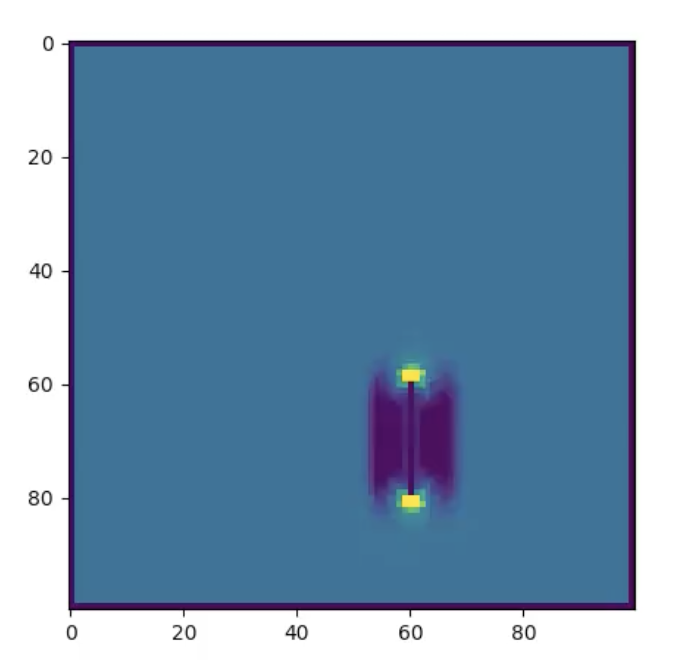
\includegraphics[width =0.6\linewidth]{plot13.png}
        \caption{$t = i$}
        \label{fig:image1}
    \end{subfigure}
    \hfill
    \begin{subfigure}[b]{0.45\textwidth}
        \centering
        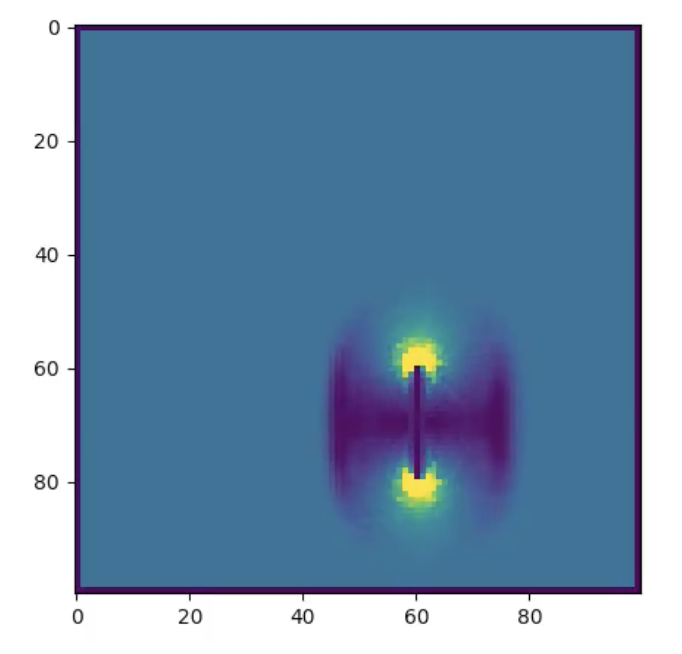
\includegraphics[width=0.6\linewidth]{plot14.png}
        \caption{$t=i+1$}
        \label{fig:image2}
    \end{subfigure}
    \vskip\baselineskip
    \begin{subfigure}[b]{0.45\textwidth}
        \centering
        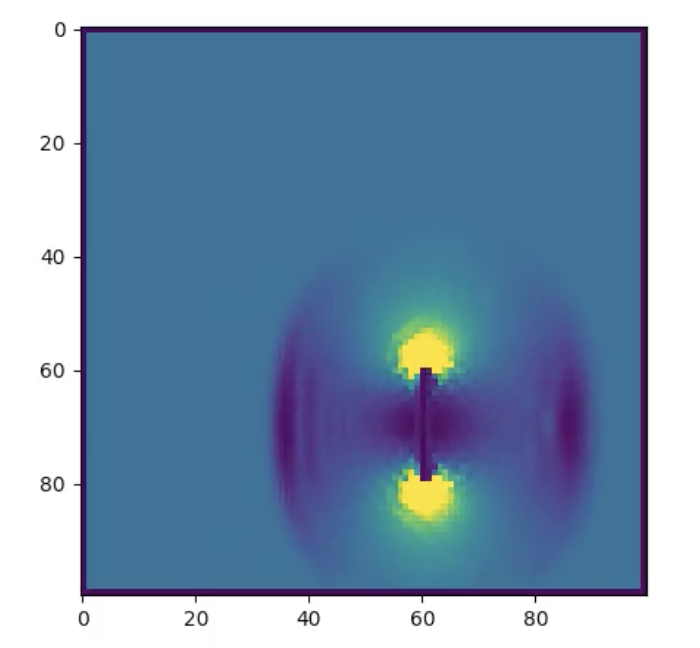
\includegraphics[width=.6\linewidth]{plot15.png}
        \caption{$t=i+2$}
        \label{fig:image3}
    \end{subfigure}
    \hfill
    \begin{subfigure}[b]{0.45\textwidth}
        \centering
        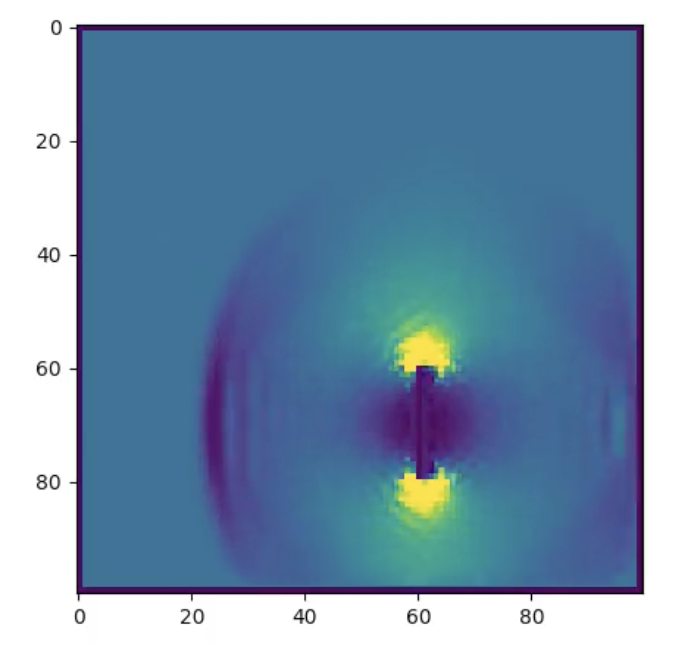
\includegraphics[width=0.6 \linewidth]{plot16.png}
        \caption{$t=i+3$}
        \label{fig:image4}
    \end{subfigure}
    \caption{LBM Simulations}
    \label{fig:images}
\end{figure}
\clearpage
\section{Industry Standard Usage - SimScale}
In this section, we will go over how to set up a simulation using an industry standard application. We will use SimScale as it requires no installation and can be run from the browser. However there are a lot of other softwares available e.g ANSYS FLUENT, OpenFOAM (Free, Open-Source). The point of this exercise is to highlight the level of technology that currenly exists at our free disposal. \cite{bib13} \\

Let us take the example of flow through a pipe junction. \\

Here are the general steps to setting up any modern CFD simulation - 
\begin{figure}[hbt!]
  \centering
  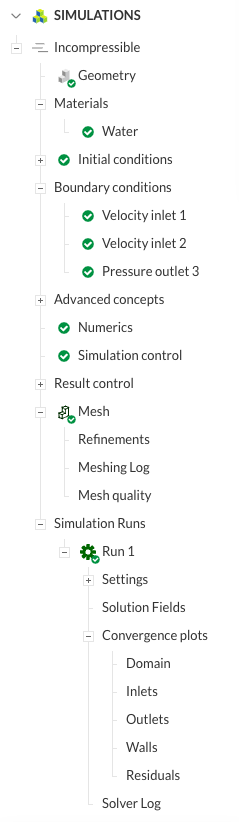
\includegraphics[width=4cm]{plot55.png}
  \caption{Modern CFD Pipeline\label{fig:fig1}}
\end{figure}
\FloatBarrier 
\begin{itemize}
    \item Geometry
    \begin{itemize}
        \item First step is always to set up the geometry. In modern CFD software this is done through uploading of CAD models of the geometry.
        \item Then defining the fluid's extent of reach needs to be done.
        \item This is how it looks in our example
        \begin{figure}[hbt!]
  \centering
  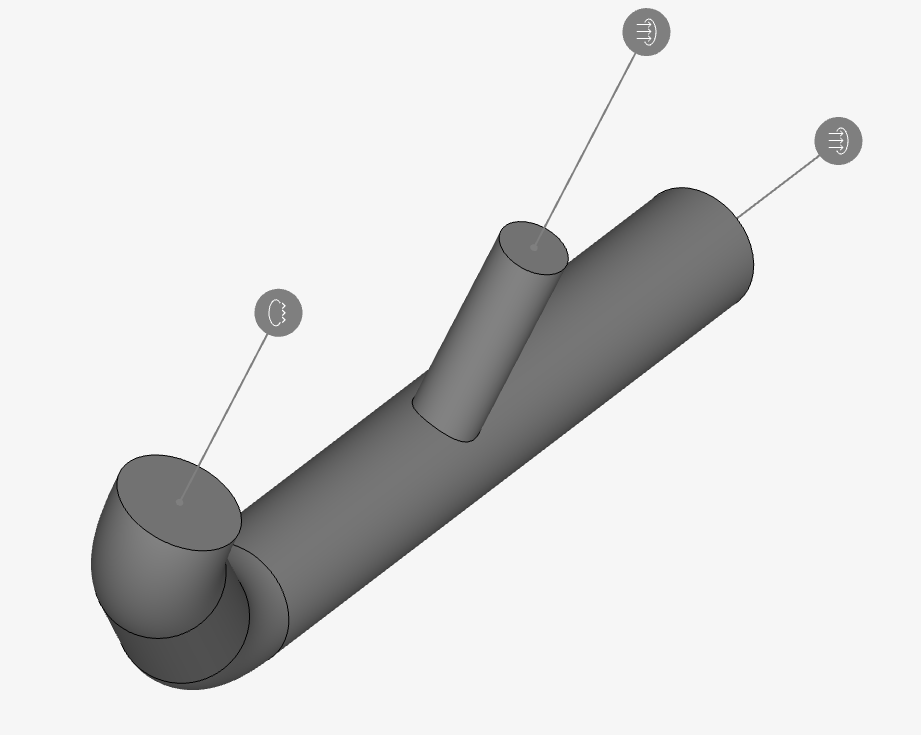
\includegraphics[width=4cm]{plot4.png}
  \caption{Plot of CAD model\label{fig:fig1}}
\end{figure}
\FloatBarrier 

\end{itemize}
    \item Flow type and Boundary Conditions
    \begin{itemize}
        \item There is an option to select the type of flow we want and in this case it is steady-state, incompressible pipe flow. We also have the option to select the material we want, in our case we will select water.
        \item We will then have to specify the boundary conditions for the given geometry.
        \item In our example, we would have to specify the velocity in the 3 open areas in the pipe, to be able to simulate.
        \begin{figure}[hbt!]
  \centering
  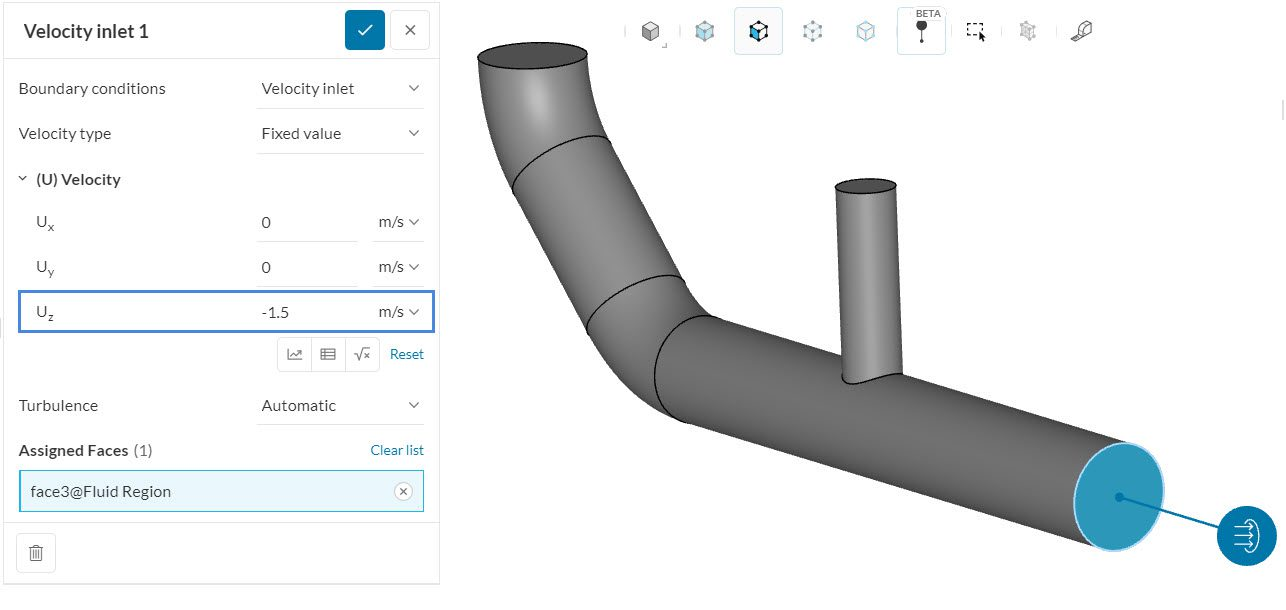
\includegraphics[width=10cm]{plot5.jpg}
  \caption{Boundary Condition set up for one inlet\label{fig:fig1}}
\end{figure}
    \end{itemize}
    \item Meshing
    \begin{itemize}
        \item We can also view and choose the type of meshing we want. In our example, we have gone with an unstructured triangular meshing.
        \begin{figure}[hbt!]
  \centering
  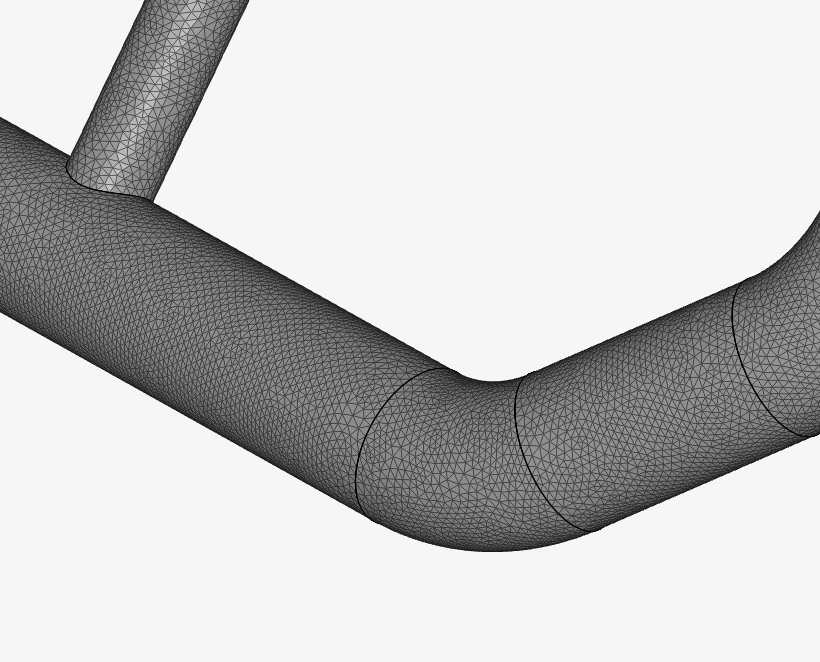
\includegraphics[width=6cm]{plot99.png}
  \caption{Meshing\label{fig:fig1}}
\end{figure}
        
    \end{itemize}
    \item Simulation and Results
    \begin{itemize}
        \item We can run the simulation with the inputs and conditions we have provided and we can analyse various things.
        \item Below is plots of velocity magnitude and pressure profiles in the pipe.
        \begin{figure}[hbt!]
\centering
\begin{subfigure}{0.4\textwidth}
  \centering
  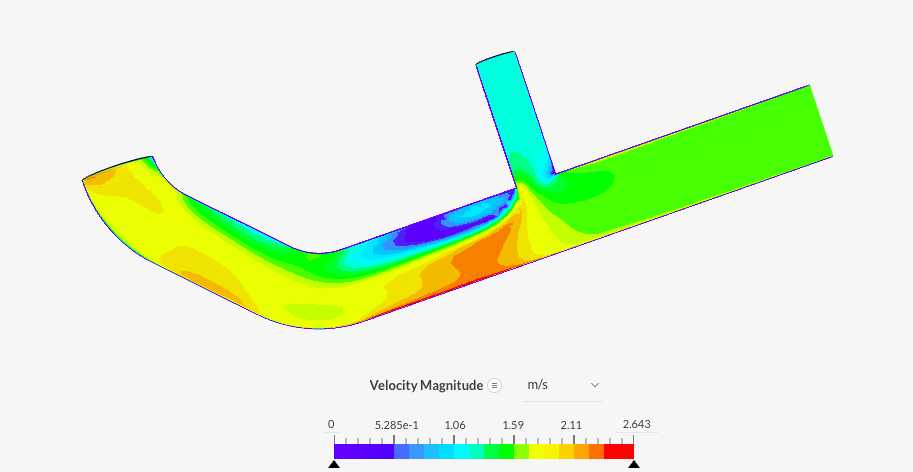
\includegraphics[width=0.9\linewidth]{plot6.png}
  \caption{Velocity Magnitude}
  \label{fig:sub1}
\end{subfigure}%
\begin{subfigure}{0.4\textwidth}
  \centering
  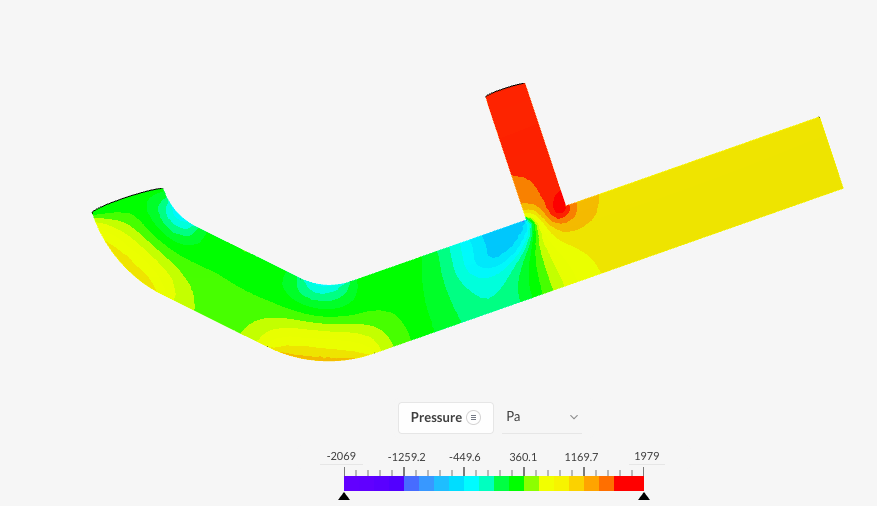
\includegraphics[width=0.9\linewidth]{plot7.png}
  \caption{Pressure Profile}
  \label{fig:sub2}
\end{subfigure}
\caption{Results of the simulation}
\label{fig:test}
\end{figure}
\FloatBarrier 
    \end{itemize}
\end{itemize}

As we can see, it is very similar to the way we approached the 1D problem.
\section{Latest Developments}
The purpose of this section is to cover the latest development in CFD research, Physics Informed Neural Networks \cite{bib14}. I am introducing this topic in hopes that readers can be inspired to carry on their learning and apply it in modern developments. 
\subsection{Physics Informed Neural Networks (PINNs)}
 Raissi et al. \cite{bib14} in their seminal work introducted the idea of physics informed neural networks. Here, the governing equations of any situation can be specified and it is used in the training process. The problem is broken down into a set of fundamental PDE's and include boundary conditions and are of the form 
 \begin{equation}
     u_{t} + N[u;\lambda] = 0, x \ \epsilon \ \Omega, t\ \epsilon \ [0, T]
 \end{equation}
The $N[u;\lambda]$ represents nonlinear operator and refers to a space in $R^{D}$. 

We will then decide the neural network architecture to move forward with, different problems require different architectures. \\

The inputs generally look like a spatial or temporal coordinates (e.g. x,y,t for 2D problem), and the output will be the field we require (e.g., temperature, pressure, velocity). \\

The algorithm resembles this order 
\begin{itemize}
    \item Decide the neural network $\hat{u}(x;\theta)$
    \item Two training sets $\tau_{f}$ and $\tau_{b}$ for equation and boundary conditions
    \item Specify loss function by adding the weighted $L^{2}$ norm of both the PDE and boundary condition forward passes.
    \item Minimise the loss $L(\theta ; \tau) = w_f L_f (\theta ; \tau_{f} + w_b L_b (\theta ; \tau_{b}))$ and find the best parameters.
\end{itemize}

\begin{figure}[hbt!]
  \centering
  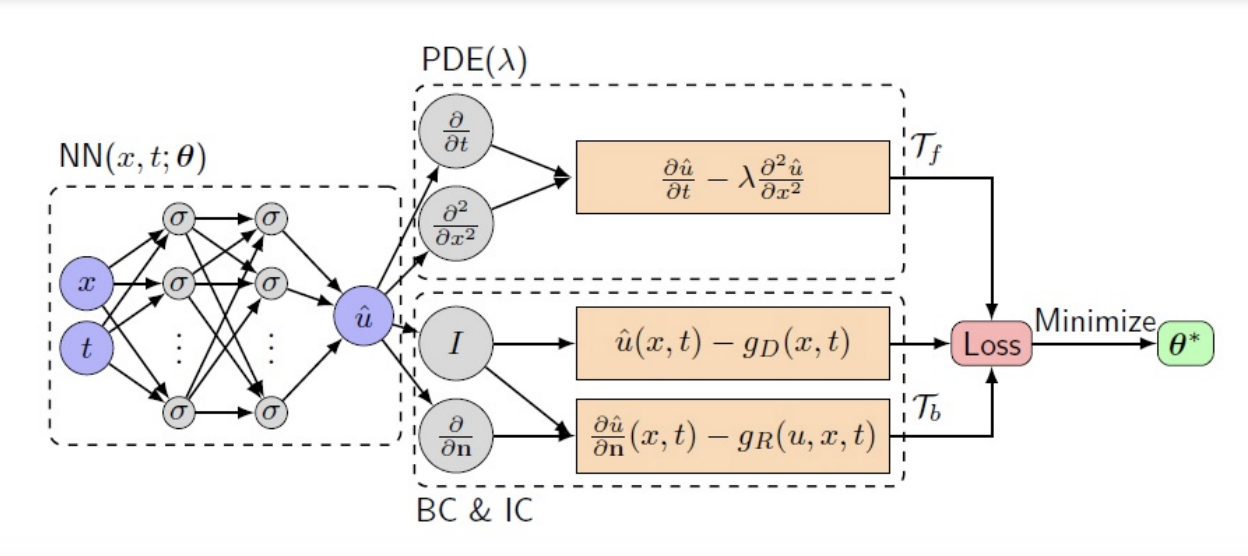
\includegraphics[width=12cm]{plot17.png}
  \caption{PINN pipeline for solving 1D diffusion problem \label{fig:fig1}}
\end{figure}
\FloatBarrier 

\printbibliography
\end{document}